\chapter{Implementación}

%%%%%%%%%%%%%%%%%%%%%%%%%%%%%%%%%%%%%%%%%
% SECCION: ENTRENAMIENTO DEL MODELO DE VISION ARTIFICIAL %
%%%%%%%%%%%%%%%%%%%%%%%%%%%%%%%%%%%%%%%%%
\section{Entrenamiento del Modelo de Visión Artificial}
\label{sec:entrenamiento_del_modelo_de_vision_artificial}

La implementación del sistema de visión artificial para la detección de residuos sólidos en cuerpos de agua requirió el entrenamiento iterativo de modelos convolucionales de alto rendimiento. Para acelerar el proceso y manejar grandes volúmenes de datos (\textit{datasets} de entrenamiento y validación), el flujo de trabajo de \textit{Machine Learning} se ejecutó en la nube utilizando la infraestructura de cómputo \textbf{Modal}. Esta plataforma permitió el aprovisionamiento bajo demanda de potentes aceleradores gráficos, específicamente \textbf{GPUs NVIDIA L40S}, logrando tiempos de convergencia sustancialmente menores en comparación con un entorno local tradicional.

Durante esta fase, se implementó un mecanismo de parada temprana (\textit{Early Stopping}) con una paciencia de 50 épocas para evitar el sobreajuste (\textit{overfitting}). Bajo esta configuración, los entrenamientos convergieron de manera óptima deteniéndose automáticamente en el momento exacto en el cual la pérdida de validación dejó de disminuir. Esta estrategia garantiza que los modelos resultantes conserven su máxima capacidad de generalización ante nuevas muestras visuales del entorno fluvial, deteniendo además el consumo de cómputo innecesario.

Con el objetivo de determinar la arquitectura más apta para el proyecto, se llevó a cabo una evaluación comparativa (\textit{benchmark}) utilizando tres variantes de la popular familia YOLO: los modelos consolidados YOLOv8 y YOLOv11, así como el modelo de vanguardia \textbf{YOLO26}.

Desarrollado por Ultralytics como la última evolución diseñada específicamente para dispositivos de borde (\textit{Edge}) y bajo consumo, YOLO26 introduce una arquitectura nativa de extremo a extremo que elimina el paso de post-procesamiento de supresión no máxima (NMS) y el módulo DFL. Además, incorpora el innovador optimizador MuSGD (un híbrido de SGD y Muon), el cual mejora la estabilidad y velocidad de convergencia del entrenamiento. En conjunto, estas optimizaciones logran una implementación significativamente más ligera y una inferencia en CPU hasta un 43\% más rápida, características idóneas para operar en sistemas con recursos limitados como el nodo concentrador del presente sistema.

%%%%%%%%%%%%%%%%%%%%%%%%%%%%%%%%%%%%%%%%%
% SUBSECCION: ANALISIS DE METRICAS DE DESEMPENO %
%%%%%%%%%%%%%%%%%%%%%%%%%%%%%%%%%%%%%%%%%
\subsection{Análisis de Métricas de Desempeño}
\label{subsec:analisis_de_metricas_de_desempeno}

El desempeño de los modelos fue evaluado utilizando métricas estándar en el ámbito de la detección de objetos: Precisión (\textit{Precision}), Sensibilidad (\textit{Recall}), Pérdida de Validación (\textit{Validation Loss}), y la Precisión Promedio Media (mAP) evaluada en un umbral de intersección sobre unión (IoU) del 50\% (mAP50) y en el rango más estricto de 50-95\% (mAP50-95).

La Figura \ref{fig:metricas_yolo_barras} ilustra la comparativa general de estos indicadores para los tres modelos entrenados.

\begin{figure}[H]
  \centering
  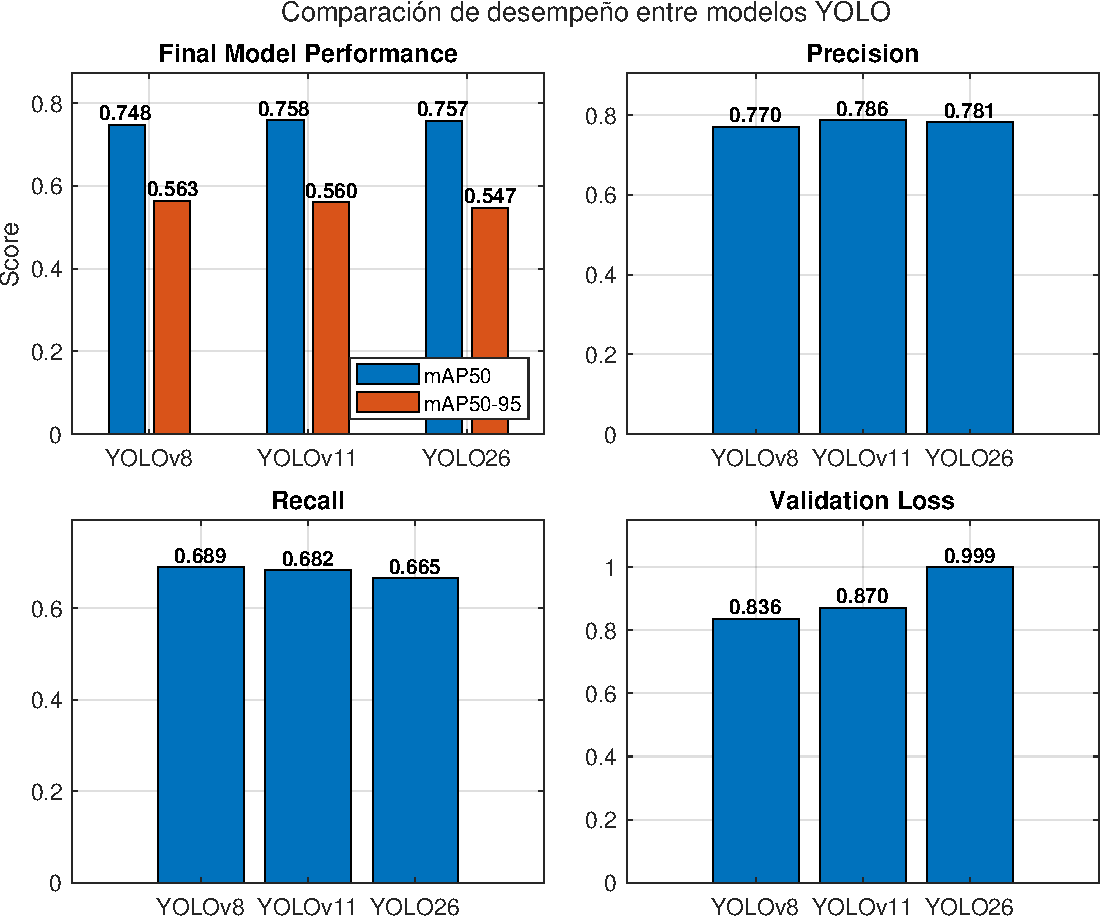
\includegraphics[width=1\linewidth]{Documento/Imagenes/Implementación/Test_yolo/bars_clean.pdf}
  \caption{Comparativa general de métricas de desempeño entre YOLOv8, YOLOv11 y YOLO26.}
  \label{fig:metricas_yolo_barras}
\end{figure}

Del análisis de la gráfica, se observa que el modelo \textbf{YOLOv8} obtuvo la Precisión más alta (\num{0.758}), indicando una tasa menor de falsos positivos en comparación con sus sucesores. Sin embargo, en la métrica de Pérdida de Validación (\textit{Validation Loss}), que refleja la capacidad de generalización del modelo frente a datos no vistos, el \textbf{YOLOv11} demostró una clara superioridad al registrar la menor pérdida (\num{0.836}), en contraste con el \num{0.999} de YOLOv8 y el \num{0.870} de YOLO26.

Para complementar esta evaluación estática, la Figura \ref{fig:metricas_yolo_map} expone la evolución dinámica del entrenamiento a lo largo de su progreso. Se grafica la convergencia del mAP50, mAP50-95, la curva Precision-Recall y la disminución de la Pérdida de Validación (\textit{Validation Loss}).

\begin{figure}[H]
  \centering
  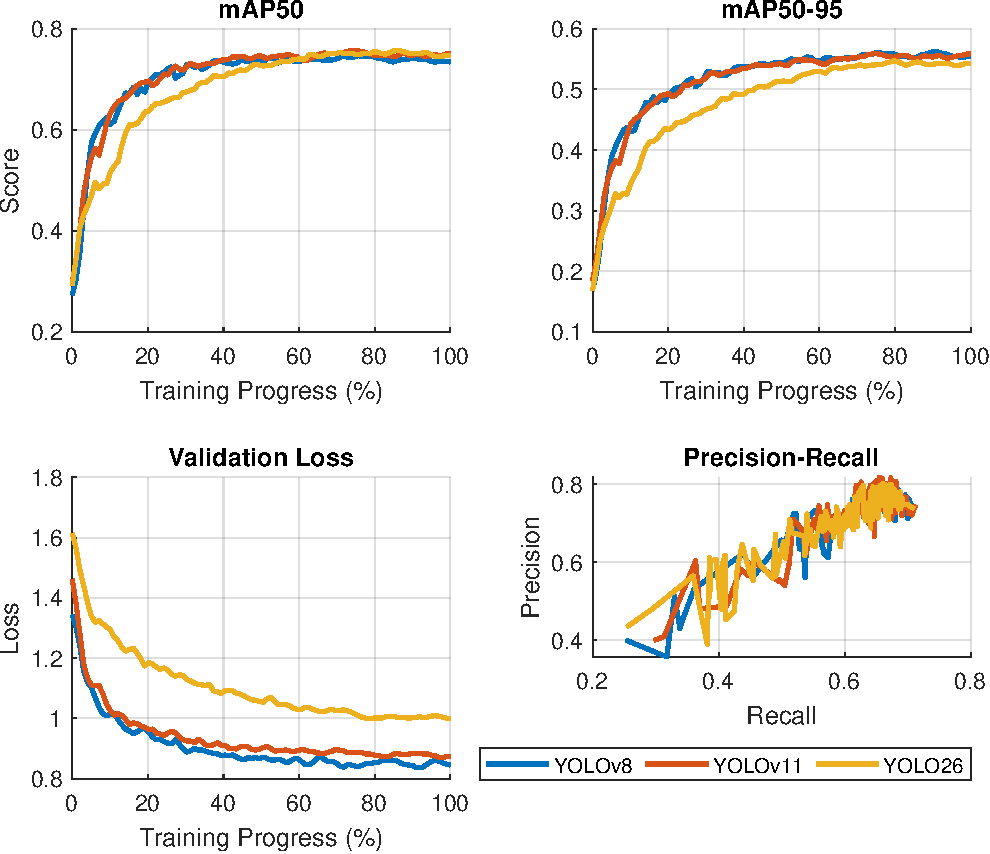
\includegraphics[width=1\linewidth]{Documento/Imagenes/Implementación/Test_yolo/comparison_main.pdf}
  \caption{Evolución de las métricas durante el progreso del entrenamiento (mAP50, mAP50-95, Curva PR y Pérdida de Validación) para YOLOv8, YOLOv11 y YOLO26.}
  \label{fig:metricas_yolo_map}
\end{figure}

De acuerdo con estas curvas de aprendizaje, \textbf{YOLOv11} no solo alcanzó el pico de rendimiento absoluto con un mAP50 de \textbf{\num{0.786}} y un mAP50-95 de \num{0.560}, sino que demostró la convergencia más estable y la menor pérdida de validación final. Le sigue muy de cerca el modelo \textbf{YOLO26}, con un mAP50 de \num{0.781}, el cual a pesar de su diseño \textit{NMS-free} para ejecución rápida en el borde, registró un rendimiento ligeramente inferior en la zona estricta de intersección (mAP50-95 de \num{0.547}). El YOLOv8 clásico cerró con \num{0.770} en mAP50.

Con base en esta implementación impulsada por la plataforma Modal, se determina que la arquitectura YOLOv11 proporciona el equilibrio óptimo entre capacidad predictiva, estabilidad de convergencia y generalización para la identificación de contaminantes superficiales en el nodo concentrador.

%%%%%%%%%%%%%%%%%%%%%%%%%%%%%%%%%%%%%%%%%
% SECCION: DESARROLLO DEL SISTEMA WEB DE MONITOREO %
%%%%%%%%%%%%%%%%%%%%%%%%%%%%%%%%%%%%%%%%%
\section{Desarrollo del Sistema Web de Monitoreo}
\label{sec:desarrollo_del_sistema_web_de_monitoreo}

Para centralizar la recepción, visualización y gestión de la telemetría recolectada por el nodo sensor, se desarrolló un Sistema Web de Monitoreo robusto. Esta plataforma fue concebida bajo una arquitectura de cliente-servidor unificada, diseñada para garantizar escalabilidad, seguridad en el acceso a la información y una experiencia de usuario fluida e interactiva.

%%%%%%%%%%%%%%%%%%%%%%%%%%%%%%%%%%%%%%%%%
% SUBSECCION: ARQUITECTURA TECNOLÓGICA %
%%%%%%%%%%%%%%%%%%%%%%%%%%%%%%%%%%%%%%%%%
\subsection{Arquitectura Tecnológica}
\label{subsec:arquitectura_tecnologica}

El núcleo de la plataforma se construyó utilizando el ecosistema de \textbf{Next.js 14}, aprovechando el paradigma de \textit{App Router}. Esta decisión arquitectónica permitió integrar tanto el \textit{Frontend} (interfaz de usuario) como el \textit{Backend} (API RESTful) en un único repositorio estructurado. El desarrollo se llevó a cabo utilizando \textbf{TypeScript} para garantizar el tipado estático estricto, reduciendo drásticamente los errores en tiempo de ejecución durante la manipulación de datos telemétricos. 

El diseño visual y la adaptabilidad para múltiples dispositivos (\textit{Responsive Design}) se implementaron a través de \textbf{Tailwind CSS v4}, un \textit{framework} de utilidades que facilitó la creación de una interfaz coherente, minimalista y ligera, sin la sobrecarga operativa de hojas de estilo monolíticas.

%%%%%%%%%%%%%%%%%%%%%%%%%%%%%%%%%%%%%%%%%
% SUBSECCION: DISEÑO DE BASE DE DATOS Y ORM %
%%%%%%%%%%%%%%%%%%%%%%%%%%%%%%%%%%%%%%%%%
\subsection{Diseño de la Base de Datos y ORM}
\label{subsec:diseno_de_la_base_de_datos_y_orm}

La persistencia de datos se gestiona mediante un motor relacional de alto rendimiento \textbf{PostgreSQL}. Para abstraer la complejidad de las consultas SQL, mitigar vulnerabilidades de inyección y mantener la sincronía perfecta entre el código fuente y el esquema de la base de datos, se incorporó la herramienta \textbf{Prisma ORM}.

El modelo relacional (\textit{schema}) fue diseñado a la medida para capturar la totalidad de la información operativa del sistema. Sus entidades núcleo abarcan:
\begin{itemize}
    \item \textbf{User}: Gestiona las credenciales de los operadores y administradores, así como sus respectivos roles de autorización.
    \item \textbf{Node}: Modela las estaciones físicas de monitoreo (nodos), almacenando su identificador criptográfico, coordenadas geográficas de despliegue y estado operativo actual.
    \item \textbf{SensorReading}: Almacena el historial cronológico de la telemetría, abarcando en cada iteración las mediciones precisas de pH, oxígeno disuelto, turbidez, conductividad eléctrica, temperatura y nivel de batería del dispositivo.
    \item \textbf{WasteDetection}: Registra los eventos críticos de contaminación superficial procesados por el modelo de visión artificial YOLO, conservando la evidencia fotográfica, el nivel de confianza de la predicción y una estimación del porcentaje de área afectada.
\end{itemize}

%%%%%%%%%%%%%%%%%%%%%%%%%%%%%%%%%%%%%%%%%
% SUBSECCION: SEGURIDAD Y VISUALIZACION %
%%%%%%%%%%%%%%%%%%%%%%%%%%%%%%%%%%%%%%%%%
\subsection{Seguridad y Visualización Telemétrica}
\label{subsec:seguridad_y_visualizacion}

Debido al carácter delicado de los datos medioambientales recopilados, el acceso a la plataforma se encuentra estrictamente protegido. La autenticación se implementó mediante el estándar \textbf{NextAuth.js}, el cual cifra y valida las credenciales de los usuarios empleando \textit{bcryptjs} antes de extender \textit{tokens} de sesión JWT para autorizar el acceso al Panel de Control (\textit{Dashboard}).

Para transformar la extensa base de datos crudos en información accionable y digerible para los operadores, la interfaz de usuario integra componentes de visualización analítica de vanguardia:
\begin{enumerate}
    \item \textbf{Geolocalización en Tiempo Real}: Mediante la integración de las librerías \textbf{Leaflet} y \textit{react-leaflet}, la plataforma renderiza un mapa interactivo global. Este componente extrae la latitud y longitud de la base de datos para posicionar marcadores de cada nodo sensor, permitiendo al usuario auditar el área de despliegue y consultar el estado general de red de un solo vistazo.
    \item \textbf{Análisis Gráfico Evolutivo}: El comportamiento histórico de la calidad del agua no se presenta en tablas estáticas, sino que se despliega mediante gráficos de series temporales altamente dinámicos construidos con \textbf{Recharts}. Esta representación visual permite a los investigadores identificar fluctuaciones inusuales, patrones cíclicos y anomalías en los parámetros fisicoquímicos a lo largo del tiempo con extrema facilidad.
\end{enumerate}

% [TODO: INSERCIÓN DE IMAGEN PENDIENTE]
% Cuando tengas las capturas de pantalla, descomenta y ajusta el siguiente bloque:
% \begin{figure}[H]
%   \centering
%   \includegraphics[width=0.9\linewidth]{Documento/Imagenes/Implementación/dashboard_monica.png}
%   \caption{Interfaz principal (Dashboard) del Sistema Web de Monitoreo.}
%   \label{fig:dashboard_web}
% \end{figure}
